% =============================================================================
% figure_captions.tex
%
% Elsevier-style captions for the manuscript figures, in figure-number order.
% Each caption is written to stand alone: what is plotted, on which population,
% which interval, and what it means, without the reader returning to the text.
% Panel letters are explained inside the caption.
%
% Figure numbering note: what was drafted as a single three-panel conservation
% figure is issued as three separate figures (5, 6, 7), because its first panel
% needs the full column width for its 12 direction labels. Lettered sub-numbers
% are reserved for panels of one figure, so they are not used here.
%
% All figures are drawn for a double-column 190 mm measure, body 9 pt, minimum
% 8 pt, vector (PDF + SVG). They are INCLUDED at \linewidth, not at 190 mm: the
% submission compiles single column under the preprint/review options, where the
% text block is about 135 mm, so a fixed 190 mm ran roughly 26 mm past each
% margin and clipped the right-hand panel. LaTeX reports no overfull box for
% this, because a centred \includegraphics wider than the line simply protrudes,
% so it is invisible to the log and to every source check.
% Every numeric value in these captions is asserted against the analysis
% outputs at figure build time: the corrected-label outputs for Figs. 3-8 (2026-09-23).
% =============================================================================

% ---------------------------------------------------------------- Figure 1 --
\begin{figure}[htbp]
  \centering
  \makebox[\linewidth][c]{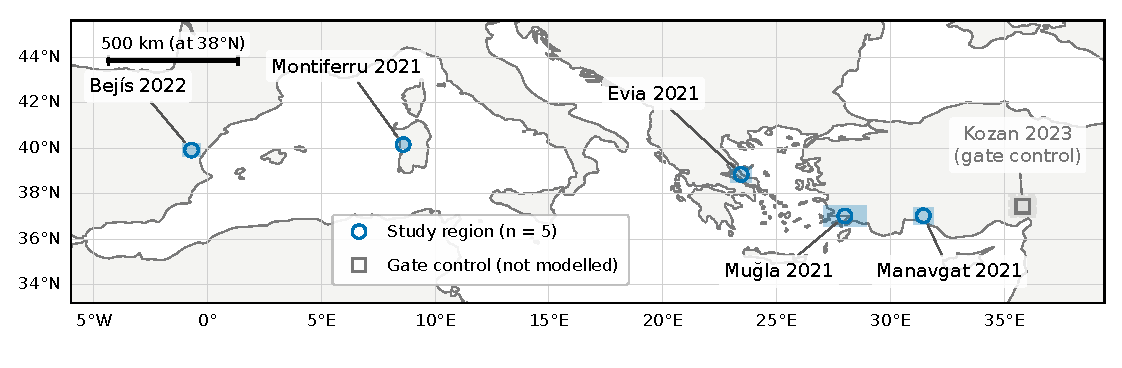
\includegraphics[width=140mm]{figures/fig1_study_map.pdf}}
  \caption{\textbf{Study regions and the gate negative control.} Locations of
  the five wildfire regions analysed in this study (blue, circular markers):
  Manavgat 2021 and Mu\u{g}la 2021 (T\"urkiye), Bej\'is 2022 (Spain), North
  Evia 2021 (Greece, extended AOI) and Montiferru 2021 (Sardinia, Italy).
  Rectangles are the true analysis areas of interest; the ring marks each
  centroid, because at basin scale the rectangles alone are hard to locate.
  Kozan 2023 (grey, dashed outline, square marker) is \emph{not} a study
  region: it is the negative control used to calibrate the burned-landcover
  admissibility gate, and it enters no model, transfer or diagnostic anywhere
  in this paper. Its rectangle is the true extent of its processed AOI and is
  larger than the study AOIs for that reason alone; the difference in size
  carries no methodological meaning and is not a design choice. Coastlines are
  Natural Earth 1:50\,m; country borders are omitted deliberately. The scale
  bar is exact only at 38\textdegree N. Region bounding boxes match Table~C1 to
  $5\times10^{-3}$ degrees.}
  \label{fig:study-map}
\end{figure}

% ---------------------------------------------------------------- Figure 2 --
\begin{figure}[htbp]
  \centering
  \makebox[\linewidth][c]{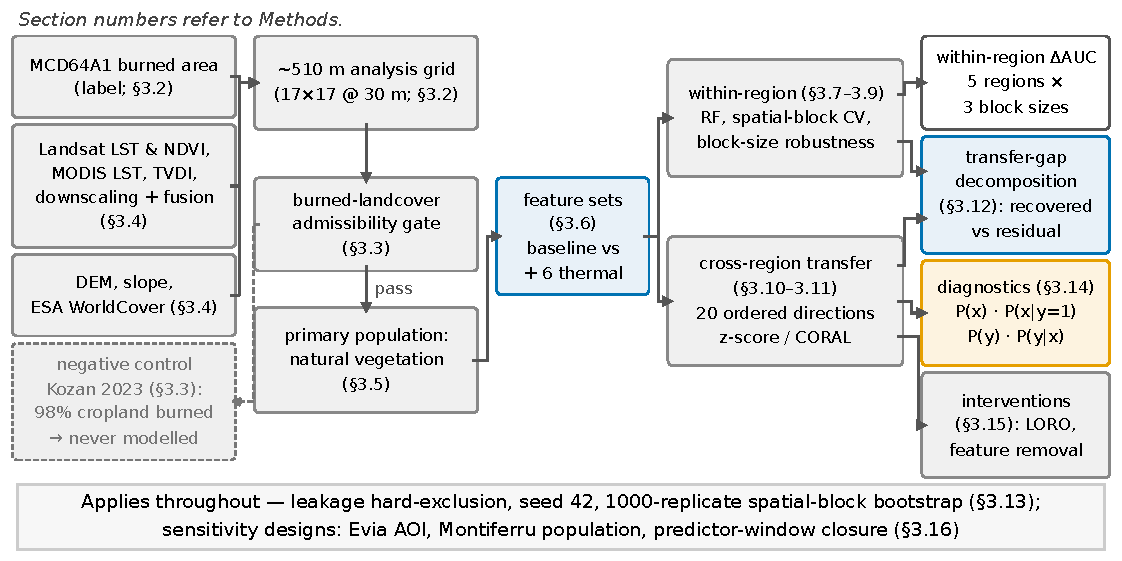
\includegraphics[width=140mm]{figures/fig2_schematic.pdf}}
  \caption{\textbf{Processing pipeline and evaluation programme.} Flow from
  source products (left) to the transfer and diagnostic programme (right);
  every box carries the Methods subsection that specifies it. The five source
  products (MCD64A1 burned area, Landsat Collection 2 Level-2, MOD11A1,
  Copernicus DEM GLO-30 and ESA WorldCover) merge onto the reconstructed
  $\sim$510\,m analysis grid
  ($17\times17$ pixels of the 30\,m reference grid). The burned-landcover
  admissibility gate has two outcomes: regions that \emph{pass} proceed to the
  natural-vegetation primary population, while the rejecting branch (grey,
  dashed) terminates in the Kozan 2023 negative control, whose burned area is
  98\% cropland and which is never modelled. The dashed connector deliberately
  carries no arrowhead onward, so the control cannot be read as entering the
  pipeline. Feature sets feed two evaluations in parallel: within-region
  (random forest under spatial-block cross-validation) and cross-region
  transfer (source-only, 20 ordered directions, with label-blind z-score and
  CORAL adaptation). Their levels are combined in the transfer-gap
  decomposition (\S3.12). The footer states what applies throughout: leakage
  hard-exclusion, seed 42, 1000-replicate spatial-block bootstrap (\S3.13), and
  the sensitivity designs (\S3.16). Section references are verified against the
  Methods heading list when the figure is built.}
  \label{fig:pipeline}
\end{figure}

% ---------------------------------------------------------------- Figure 3 --
\begin{figure}[htbp]
  \centering
  \makebox[\linewidth][c]{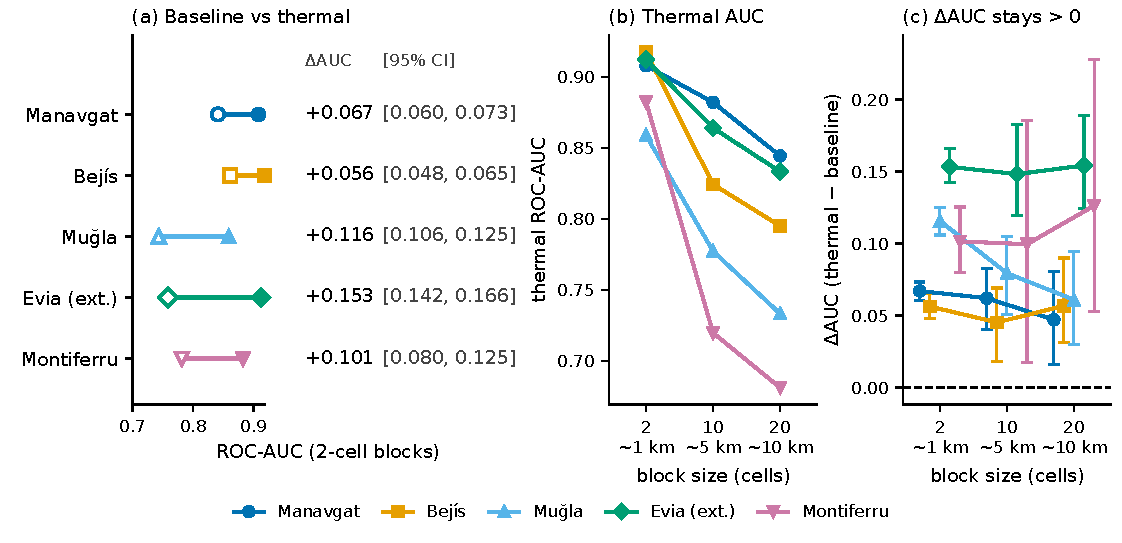
\includegraphics[width=140mm]{figures/fig3_within_robustness.pdf}}
  \caption{\textbf{The thermal increment replicates in all five regions and
  survives coarser spatial blocking.} Natural-vegetation primary population;
  random forest with the primary weighted configuration; all intervals are
  95\% spatial-block bootstrap intervals (1000 replicates, seed 42).
  \textbf{(a)} Baseline versus thermal out-of-fold ROC-AUC per region at the
  default 2-cell ($\sim$1\,km) blocking: the open marker is the static baseline
  feature set, the filled marker is the baseline plus the six thermal
  predictors, and the connecting bar is the increment. The right-hand column
  reports the paired $\Delta$AUC and its 95\% interval; it is a fixed column
  placed beyond the plotted AUC range, so no label position depends on a data
  value. Every interval excludes zero. \textbf{(b)} Absolute thermal ROC-AUC
  against spatial block size (2, 10 and 20 cells, $\approx$1, 5 and 10\,km):
  absolute skill falls as blocking coarsens, in every region.
  \textbf{(c)} The thermal increment $\Delta$AUC against the same block sizes,
  with 95\% intervals: the increment does \emph{not} melt away, and its
  interval excludes zero in all ten of the 2- and 10-cell region--block-size
  combinations. The five 20-cell intervals also lie above zero but rest on 6 to
  33 positive-carrying blocks each, so they are plotted as indicative rather
  than as intervals (Table~\ref{tab:1}, table note). In (c)
  the five regions are offset horizontally by 0.15 cell so their whiskers
  separate; \textbf{this offset is cosmetic, since all five regions are evaluated
  at exactly the same three block sizes} (2, 10, 20 cells), and the offset is
  smaller than half the spacing between block sizes, so the groups cannot
  merge. Colour and marker shape both encode region, so the panels remain
  readable in greyscale.}
  \label{fig:within-robustness}
\end{figure}

% ---------------------------------------------------------------- Figure 4 --
\begin{figure}[htbp]
  \centering
  \makebox[\linewidth][c]{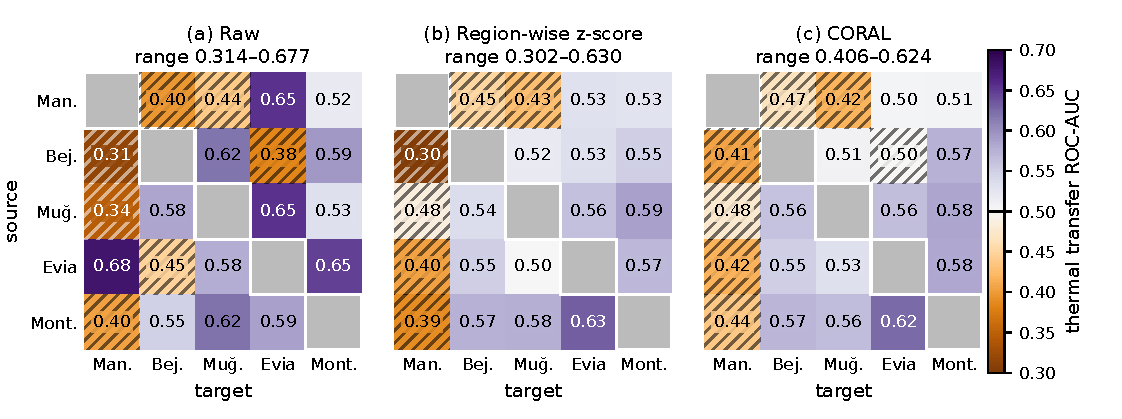
\includegraphics[width=140mm]{figures/fig4_transfer_matrix.pdf}}
  \caption{\textbf{Cross-region transfer, and what label-blind adaptation does
  to it.} Thermal transfer ROC-AUC for all 20 ordered source--target
  directions among the five regions, natural-vegetation primary population.
  \textbf{(a)} Raw transfer, no adaptation. \textbf{(b)} After region-wise
  z-score standardisation. \textbf{(c)} After CORAL. Rows are the source
  region, columns the target; the grey diagonal is within-region performance
  and is \emph{not} a transfer result. The diverging colour scale is centred
  exactly on chance (0.5, marked by the black rule on the colour bar), so
  orange is below chance and purple above. Each panel header states that
  panel's range: adaptation narrows the spread from 0.314--0.677 (raw) to
  0.302--0.630 (z-score) and 0.406--0.624 (CORAL). It compresses the matrix
  toward chance rather than lifting transfer, with one exception at the low end:
  under z-scoring Bej\'is$\rightarrow$Manavgat moves further below chance
  (0.314 to 0.302). Cells below chance are hatched.
  The hatch is a redundant cue for print: a diverging palette is symmetric in
  luminance about its centre, so in greyscale a below-chance cell would
  otherwise be indistinguishable from an equally distant above-chance one.
  Hatching follows the \emph{exact} value while the printed label is rounded to
  two decimals, so three cells print ``0.50'' with different hatching: CORAL
  Bej\'is$\rightarrow$Evia is 0.4991 (hatched, below chance), while z-score
  Evia$\rightarrow$Mu\u{g}la is 0.5013 and CORAL Manavgat$\rightarrow$Evia
  0.5043 (both un-hatched, above chance). Every cell carries its value, and
  every label's colour is chosen by measured WCAG contrast against that cell's
  rendered colour (worst case 4.6:1). Confidence intervals for these directions
  are given in Table~B9. Manavgat directions are on the corrected label
  (Section~\ref{sec:3.2}).}
  \label{fig:transfer-matrix}
\end{figure}

% ---------------------------------------------------------------- Figure 5 --
\begin{figure}[htbp]
  \centering
  \makebox[\linewidth][c]{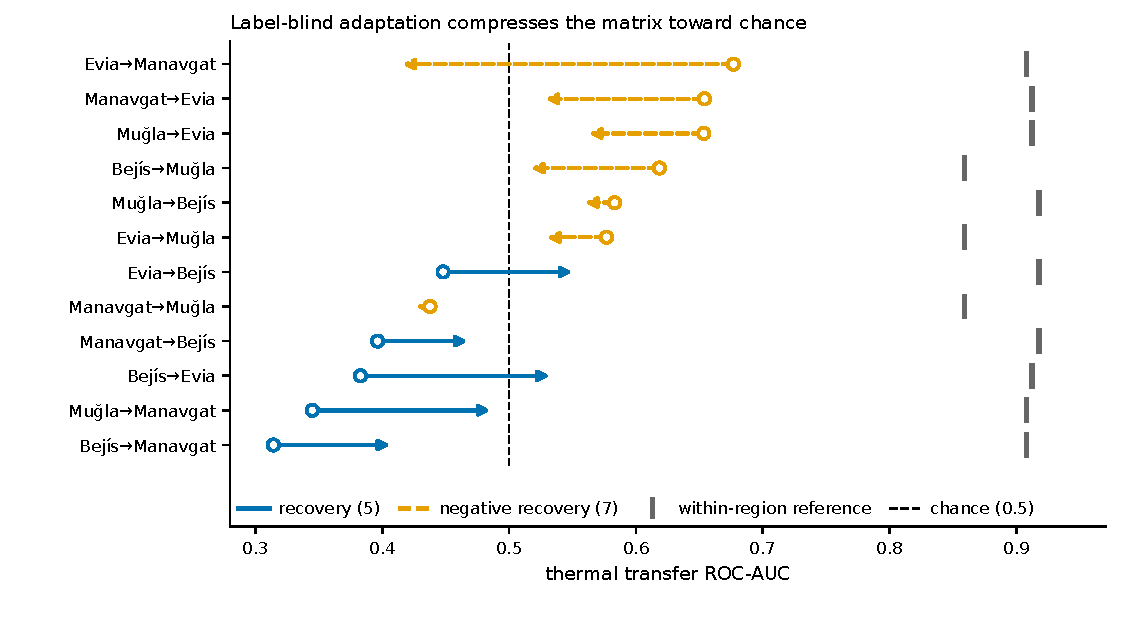
\includegraphics[width=140mm]{figures/fig5_adaptation.pdf}}
  \caption{\textbf{Label-blind adaptation compresses the matrix toward chance.}
  All 12 ordered directions among the four regions carrying the full
  decomposition (Manavgat, Bej\'is, Mu\u{g}la, Evia), natural-vegetation primary
  population. Each row is one direction. The open circle is raw transfer ROC-AUC
  and the arrow runs to the best label-blind adapted result for that direction
  (region-wise z-score or CORAL, whichever is better); the grey vertical tick is
  the within-region reference for that target, and the dashed vertical rule is
  chance. \textbf{Solid blue arrows are the five directions where adaptation
  moves transfer toward the within-region reference (recovery); dashed orange
  arrows are the seven where it moves \emph{away} from it (negative recovery).}
  Line style and colour both encode this class, because the two hues differ by
  only 2.30:1 in relative luminance and would nearly merge in greyscale. All six
  directions starting above chance are pushed down, and five of the six
  starting below chance are pushed up, so eleven of twelve end closer to chance
  and adaptation acts on the spread rather than on skill. The exception is
  Manavgat$\rightarrow$Mu\u{g}la, which starts below chance at 0.438 and is
  pushed further down to 0.427. Bej\'is$\rightarrow$Manavgat is drawn as a
  recovery because its better method, CORAL, lifts it from 0.314 to 0.406; its
  z-score arm alone moves further below chance, to 0.302 (Fig.~\ref{fig:transfer-matrix}).
  The worst case is Evia$\rightarrow$Manavgat, where raw transfer of 0.677 is
  dragged down to 0.417 against a within-region reference of 0.908, a recovered
  fraction of $-1.126$. No arrow reaches its within-region tick. Manavgat
  directions are on the corrected label (Section~\ref{sec:3.2}).}
  \label{fig:adaptation}
\end{figure}

% ---------------------------------------------------------------- Figure 6 --
\begin{figure}[htbp]
  \centering
  \makebox[\linewidth][c]{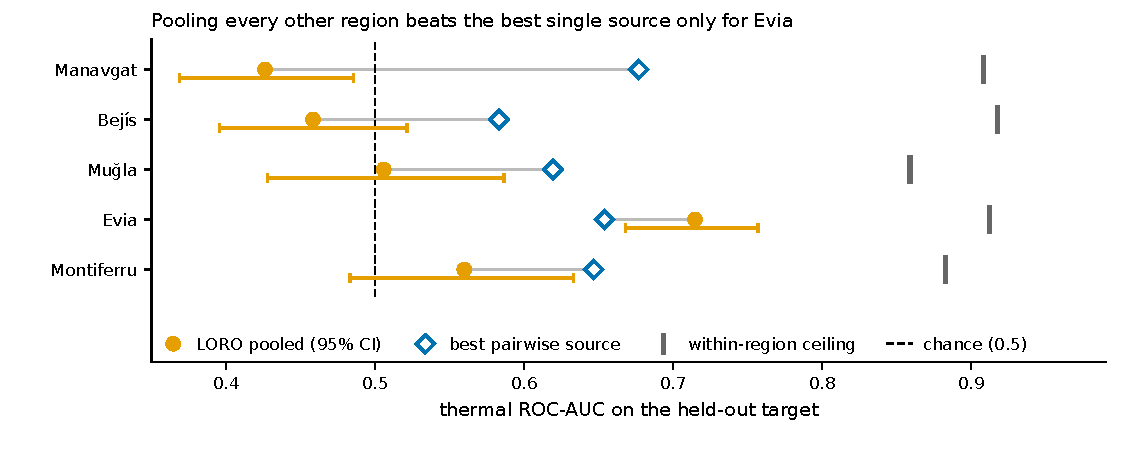
\includegraphics[width=140mm]{figures/fig6_loro.pdf}}
  \caption{\textbf{Pooling every other region does not beat the best single
  source for four of five targets.} Leave-one-region-out evaluation: for each held-out target region
  (rows), a model trained on the pooled remaining four regions (filled orange
  circle, with its 95\% spatial-block ($\approx$5\,km) bootstrap interval drawn
  just below the row) is compared against the best individual source region for
  that same
  target (open blue diamond), with the within-region ceiling as a grey vertical
  tick and chance as the dashed rule. Natural-vegetation primary population,
  thermal feature set, no adaptation. The pooled model lies to the left of the best pairwise source in four
  targets. For Evia it lies to the right, at 0.715 [0.668, 0.757] against 0.654
  for the best single source, Manavgat (Section~\ref{sec:5.3}). Elsewhere, adding
  source regions does not accumulate transferable signal. In two targets the
  pooled model falls \emph{below chance} at the point estimate (Manavgat 0.426,
  Bej\'is 0.458), and only for Manavgat does the interval lie entirely below
  chance, while a single well-chosen source reaches 0.677 and 0.583
  respectively. Every point remains far below the within-region ceiling.
  Manavgat values are on the corrected label (Section~\ref{sec:3.2}).}
  \label{fig:loro}
\end{figure}

% ---------------------------------------------------------------- Figure 7 --
\begin{figure}[htbp]
  \centering
  \makebox[\linewidth][c]{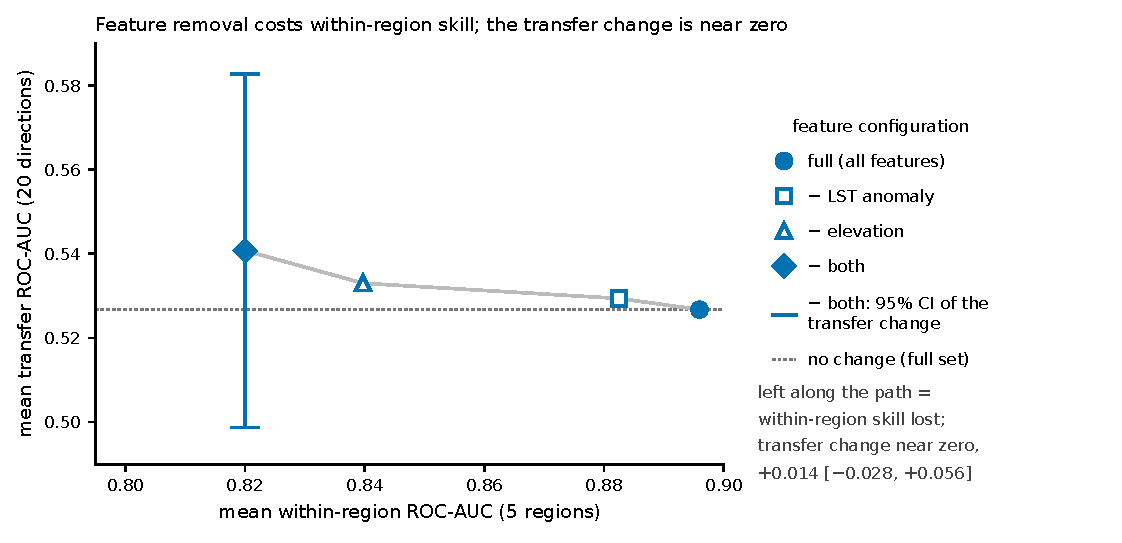
\includegraphics[width=140mm]{figures/fig7_feature_drop.pdf}}
  \caption{\textbf{Removing the direction-reversing features costs locally and
  returns nothing measurable on transfer.} Mean within-region ROC-AUC across the five regions (horizontal)
  against mean transfer ROC-AUC across the 20 ordered directions (vertical),
  for four feature configurations: the full thermal set, the set without the
  LST anomaly, without elevation, and without both. Each configuration has its
  own marker and is named in the key; the grey path connects them in that
  order. Moving left along the path, within-region skill falls monotonically
  (0.896 $\rightarrow$ 0.820) while the transfer mean rises monotonically
  (0.527 $\rightarrow$ 0.541). Both monotonicities are verified when the figure
  is built. The within-region cost is 0.076 AUC and is supported in every region.
  The change in transfer is near zero: $+$0.014 AUC, with a pair-$t$ interval
  over the ten region pairs of [$-$0.028, $+$0.056] that spans zero. No exchange
  between the two is demonstrated, since a local cost is measured and no
  compensating transfer gain is. The vertical whisker at the ``without both''
  point is that interval, drawn about the full-set transfer level (dotted line,
  no change), so its crossing of the no-change level can be read directly.
  Manavgat values are on the corrected label (Section~\ref{sec:3.2}).}
  \label{fig:feature-drop}
\end{figure}

% ---------------------------------------------------------------- Figure 8 --
\begin{figure}[htbp]
  \centering
  \makebox[\linewidth][c]{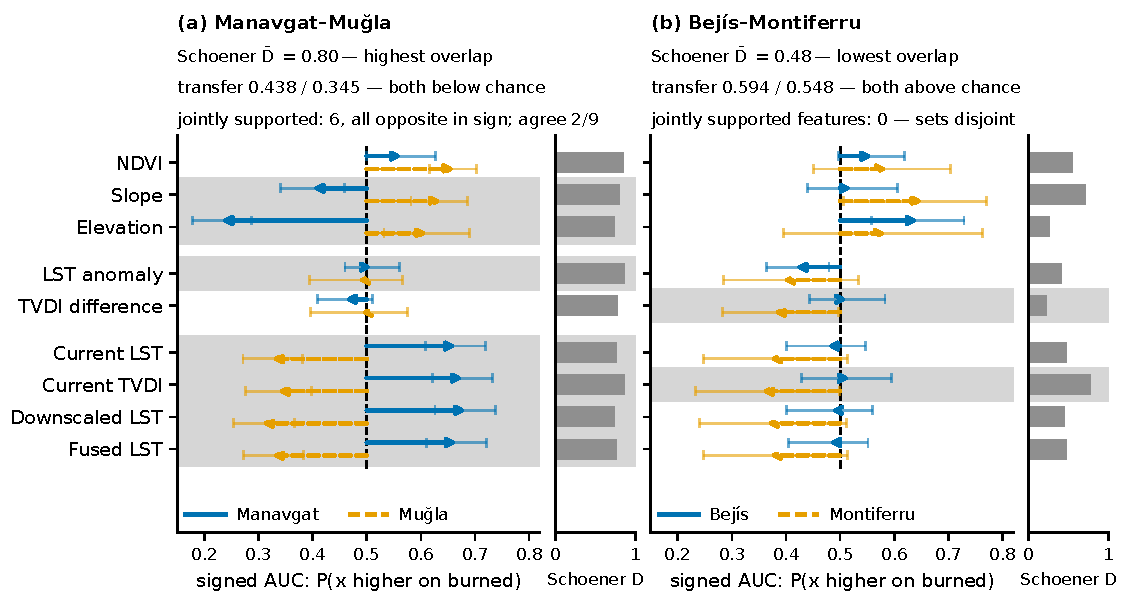
\includegraphics[width=140mm]{figures/fig8_contrast_pairs.pdf}}
  \caption{\textbf{The contrast pairs.} \textbf{(a)} Manavgat--Mu\u{g}la, the
  pair whose burned cells overlap most in environmental space (mean Schoener
  $\bar{D}=0.80$, rank 1 of 10 on all five overlap measures), transfers below
  chance in both directions at the point estimates (0.438 and 0.345).
  \textbf{(b)} Bej\'is--Montiferru, the pair that overlaps least
  ($\bar{D}=0.48$, rank 10), transfers above chance in both directions at the
  point estimates (0.594 and 0.548). Arrows run from 0.5 to each region's
  signed univariate AUC, the probability that a predictor takes a higher value
  on a burned cell than on an unburned one. A filled head marks a 95\%
  spatial-block (10-cell, $\approx$5\,km) bootstrap interval that excludes 0.5;
  an open head marks one that does not. Solid blue is the first region named,
  dashed orange the second; line style is included because the two hues nearly
  merge in greyscale. Shaded rows mark features whose sign differs between the
  two regions, and side bars give Schoener's $D$ per feature. In (a), six
  features are interval-supported in both regions, and all six have opposite
  signs; the signs agree on 2 of 9 features overall. In (b) the two supported
  sets do not intersect, and the signs agree on 7 of 9. The transfer verdicts use
  the 1\,km bootstrap, under which all four directions are off chance. At 5\,km
  blocking only Mu\u{g}la $\rightarrow$ Manavgat stays interval-supported, which
  is why the contrast is stated at the point estimates. Manavgat values are on
  the corrected label (Section~\ref{sec:3.2}).}
  \label{fig:contrast-pairs}
\end{figure}
